\section{Konstruktion eines GAHMM}

In diesem Kapitel werde ich beschreiben wie man einen Genetischen Algorithmus 
für Hidden Markov Modelle erstellen kann und dann auf die in meiner Arbeit verwendeten 
konkreten Implementationen der genetischen Operatoren eingehen.



\subsection*{Representation}
Ähnlich wie in den Papers [hier papers einfügen] 
Ist die Chromosonale Representation eines HMMs ein Vektor welcher 
die Reihen aller Matrizen hintereinander enthält.

Um die Struktur von nicht ergodischen Hidden Markov Modellen im Mutations-schritt nicht zu Verändern 
muss man die Gene Welche Startwahrscheinlichkeiten und Transitionswahrscheinlichkeiten
beschreiben von der Mutation ausschließen oder man kann eine Maske definieren
welche eine Mutation Gene welche initial 0 oder 1 sind verhindert.


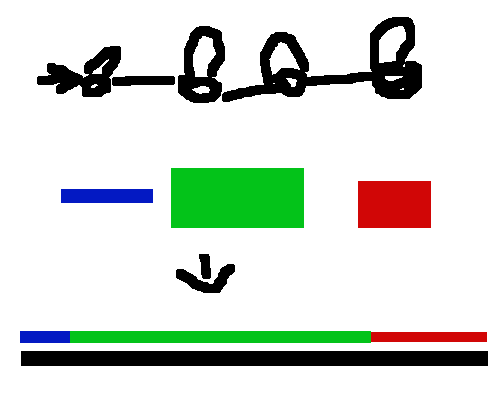
\includegraphics[scale=1.0]{images/Hmm_Chromosom_Representation.png}


\subsection*{Fitness Operator}
Die Fitness eines Chromosoms ist die durchschnittliche Log Wahrscheinlichkeit 
des Hidden Markov Models, welchen das Chromosom representiert.
Als Observations Sequenzen werden Äußerungen der Zahl 0 aus dem Free Spoken Digit Dataset verwendet

\subsection*{Mutationsoperatoren}
Mutationsoperatoren wird dies das annanas gewählt


Belegung der Parameter:

Hidden Markov Parameter 
Bei den Hidden Markov Modellen welche von den genetischen Algorithmus optimiert werden handelt es sich 
ausschließlich um Left-right Modelle mit 4 Zuständen und 128 Observationssymbolen.
Diese Werte sind relativ Arbiträr gewählt und orientieren sich an existierender Literatur zu Spracherkennung mit Hidden Markov modellen.

Als Observations-Sequenzen werden Äußerungen der Zahl 0 aus der Free Spoken Digit Database gewählt.
Welche mittels eines k-means algorithmus mit k=128 quantisiert wurden.


Genetischer Algorithmus Parameter:

Die Populationsgröße wird auf 50 beschränkt und die Anzahl der Generationen auf 100.
Das Rational für diese Entscheidung ist, dass ein Ablauf des Genetischen Algorithmus mit diesen Parametern
auf meinem Klapprechner in unter 5 minuten abläuft und 100 Generationen meißt ausreichen um den Genetischen Algorithmus konvergieren zu lassen
Die Anzahl der Observationssequenzen ist 10


\subsection*{Erweiterung des GA}
- Der genetische Algorithmus muss um einen Normalisierungsschritt erweitert werden, 
falls die Crossover oder Mutationsoperatoren keine Reihenstochastizität garantieren.